\documentclass[aps,twocolumn,secnumarabic,nobalancelastpage,amsmath,amssymb,
nofootinbib,superscriptaddress]{revtex4-1}


\usepackage{graphics}       % standard graphics specifications
\usepackage{graphicx}       % alternative graphics specifications
\usepackage{longtable}      % helps with long table options
\usepackage{url}            % for on-line citations
\usepackage{bm}             % special 'bold-math' package
\usepackage[ngerman]{babel} % deutsche Siblentrennung
\usepackage[utf8]{inputenc} % Umlaute

\def\andname{\hspace*{-0.5em},} % definiert die Trennung zwischen 2 Autoren neu

% Titelseite
\begin{document}
\title{Compton-Effekt}
\author         {Ch. Egerland}
\email[Email: ]{egerlanc@physik.hu-berlin.de}
\author         {M. Pfeifer}
\email[Email: ]{mpfeifer@physik.hu-berlin.de}
\affiliation    {Humboldt-Universität zu Berlin, Institut für Physik}
\date[Versuchsdatum: ]{13.06.2017}

%%%%%%%%%%%%%%%%%%%%%%%%%%%%%%%%%%%%%%%%%%%%%%%%%%%%%%%%%%%%%%%%%%%%%%%%%%%%%%%%
\begin{abstract}
  Lorem ipsum dolor sit amet, consectetur adipiscing elit. Nam id facilisis ligula,
  a ultrices nibh. Nullam suscipit tellus nec mauris fermentum, ornare luctus neque
  tincidunt. Aenean commodo tincidunt varius. Phasellus faucibus metus non erat
  consectetur bibendum. Duis et luctus risus, at egestas justo. Nunc eleifend lacus
  ac laoreet scelerisque. Aenean cursus dignissim magna in ultrices. In eget nisl
  quis nisi.
\end{abstract}


\maketitle


%%%%%%%%%%%%%%%%%%%%%%%%%%%%%%%%%%%%%%%%%%%%%%%%%%%%%%%%%%%%%%%%%%%%%%%%%%%%%%%%

\section{Zur Theorie des Compton-Effektes}
Der Compton-Effekt ist ein Phänomen, welches bei der Streuung von Photonen an
Teilchen beobachtet wird. Hierbei gibt das Photon einen Teil seiner Energie an das
ruhende Teilchen ab, wodurch die Wellenlänge des Photons steigt und das Teilchen
sich bewegt. Dieser Mechanismus ist in Abbildung~\ref{fig:kinematik} veranschaulicht.
Die Energie des gestreuten $\gamma$-Quants ist gegeben durch:

  \begin{equation}
    E^* = \frac{E_0}{1+\gamma(1- cos \theta)}
    \label{eq:streuenergie}
  \end{equation}

Hierbei ist $\theta$ der Streuwinkel und $\gamma = E_0/mc^2$ das Verhältnis der
Energie des eintreffenden Photons zur Ruheenergie des Elektrons. Man sieht, dass
dieser Effekt sich erst für hohe Photonenergien (also $\gamma >> 1$) bemerkbar
macht.

\begin{figure}[h]
  \centering
  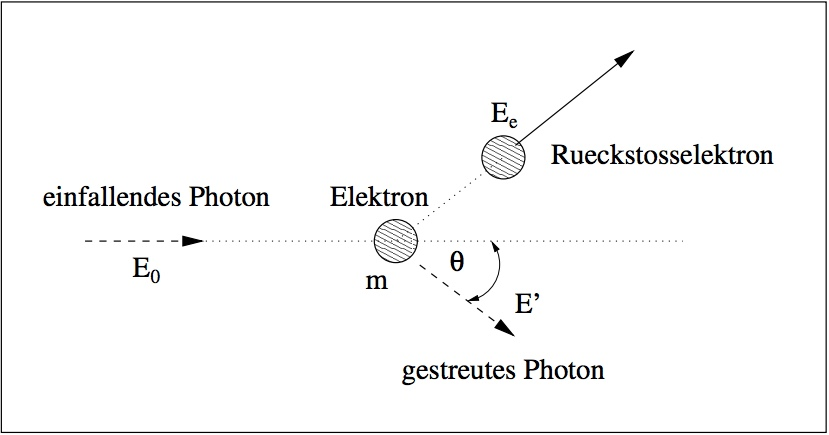
\includegraphics[width=0.5\textwidth]{comptstreu_schema.jpeg}
  \caption{\label{fig:kinematik} Kinematik des Compton-Effekts aus \cite{skript07}.}
\end{figure}

Der korrekte differentielle Wirkungsquerschnitt, der die Winkelverteilung des
Compton-Effektes beschreibt, ist durch die Klein-Nishina-Formel gegeben:

  \begin{equation}
    \frac{d \sigma}{d \Omega} = \frac{r_0^2}{2} \left( \frac{E^*}{E_0} \right)^2
    \left( \frac{E_0}{E^*} + \frac{E^*}{E_0} - sin^2 \theta    \right)
    \label{eq:kleinnishina}
  \end{equation}

Aus dieser Formel folgt, dass es eine Vorwärts-Rückwärts-Asymmetrie gibt, d.h.
es werden mehr Photonen in die Vorwärtsrichtung, als in die Rückwärtsrichtung
gestreut.


%%%%%%%%%%%%%%%%%%%%%%%%%%%%%%%%%%%%%%%%%%%%%%%%%%%%%%%%%%%%%%%%%%%%%%%%%%%%%%%%
\section{Experiment}
Der Versuchsaufbau ist in Abbildung ~\ref{fig:aufbau} gezeigt. Die Photonen treten
aus der Strahlungsquelle (Daten in Tabelle ~\ref{tab:materialien}) in den Kolliminator
welcher dafür sorgt, dass die Photonen aus nahezu 0° kommen. Das Aluminium-Streutarget
ist herausnehmbar. Dann wird die Energie der Photonen in einem Thallium dotierten
NaJ-Szintillator in Spannung umgewandelt und nach Verstärkung am PC in der Software
MAESTRO in einem Histogramm dargestellt. Die Auswertung dessen ist in Abschnitt
III besprochen.

\begin{figure}[h]
  \centering
  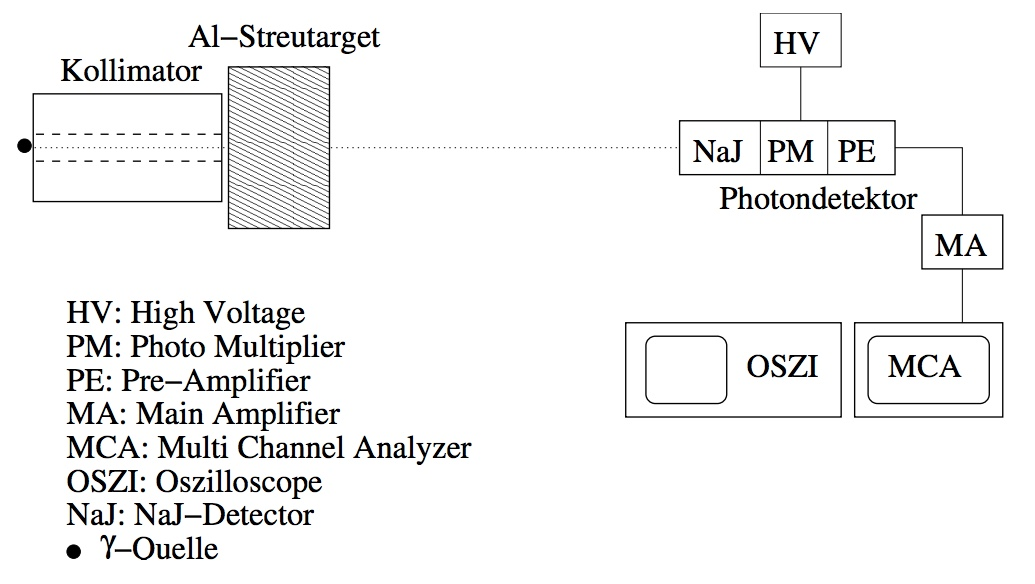
\includegraphics[width=0.5\textwidth]{aufbau.jpeg}
  \caption{\label{fig:aufbau} Versuchsaufbau aus \cite{skript07}.}
\end{figure}

\begin{table}[h]
\begin{ruledtabular}
\begin{tabular}{cccc}
 Präparat & $\gamma$-Energie in MeV & Aktivität (kBq) & Halbwertszeit\\
\hline
^{133} Ba & 0.356 & 397 & 10.54a \\
^{22} Na & 0.511 & 374 & 2.603a \\
^{137} Cs & 0.662 & 371 & 30.17a \\
\end{tabular}
\end{ruledtabular}
\caption{\label{tab:materialien} Daten der Photonenquellen ermittelt am 01.11.1996
mit einem Fehler von 4\%.}
\end{table}



%%%%%%%%%%%%%%%%%%%%%%%%%%%%%%%%%%%%%%%%%%%%%%%%%%%%%%%%%%%%%%%%%%%%%%%%%%%%%%%%
\section{Daten und Analyse}

Lorem ipsum dolor sit amet, consectetur adipiscing elit. Nam id facilisis ligula,
a ultrices nibh. Nullam suscipit tellus nec mauris fermentum, ornare luctus neque
tincidunt. Aenean commodo tincidunt varius. Phasellus faucibus metus non erat
consectetur bibendum. Duis et luctus risus, at egestas justo. Nunc eleifend lacus
ac laoreet scelerisque. Aenean cursus dignissim magna in ultrices. In eget nisl
quis nisi. Tabelle \ref{tab:table1}:







%%%%%%%%%%%%%%%%%%%%%%%%%%%%%%%%%%%%%%%%%%%%%%%%%%%%%%%%%%%%%%%%%%%%%%%%%%%%%%%%
\section{Schlussfolgerung}

Schlussoflgerung, sollten wir mal was von nem Buch oder so entnehmen nutzen wir:


\begin{quote}
  Ein Zitat mit Referenz auf das Buch\cite{melissinos1966}
\end{quote}

Lorem ipsum dolor sit amet, consectetur adipiscing elit. Nam id facilisis ligula,
a ultrices nibh. Nullam suscipit tellus nec mauris fermentum, ornare luctus neque
tincidunt. Aenean commodo tincidunt varius. Phasellus faucibus metus non erat
consectetur bibendum. Duis et luctus risus, at egestas justo. Nunc eleifend lacus
ac laoreet scelerisque. Aenean cursus dignissim magna in ultrices. In eget nisl
quis nisi.


%%%%%%%%%%%%%%%%%%%%%%%%%%%%%%%%%%%%%%%%%%%%%%%%%%%%%%%%%%%%%%%%%%%%%%%%%%%%%%%%
\bibliography{sample-paper}
\bibliographystyle{prsty}
\begin{thebibliography}{99}
\bibitem{skript07}O.Epler, U. Schwanke, Compton-Effekt (Versuchsskript),  [2007]
\bibitem{abkuerzung2}Autor, Titel, Verlag,  [1945]
\bibitem{abkuerzung3}Autor, Titel, Verlag,  [1945]
\bibitem{abkuerzung4}Autor, Titel, Verlag,  [1945]
\end{thebibliography}


%%%%%%%%%%%%%%%%%%%%%%%%%%%%%%%%%%%%%%%%%%%%%%%%%%%%%%%%%%%%%%%%%%%%%%%%%%%%%%%%
\clearpage
\appendix

\section{Sonstiges}
Hier sehen wir einen Beispiel Anhang und so könnte man Code in Latex einbinden:
\begin{verbatim}
> mkdir ~/8.13
> mkdir ~/8.13/papers
> mkdir ~/8.13/papers/template
> cd ~/8.13/papers/template
\end{verbatim}


%%%%%%%%%%%%%%%%%%%%%%%%%%%%%%%%%%%%%%%%%%%%%%%%%%%%%%%%%%%%%%%%%%%%%%%%%%%%%%%%


\end{document}
